\documentclass{llncs}

\pdfpagesattr{/CropBox [92 72 523 738]} % LNCS page: 152x235 mm

% Define a version of \paragraph whose heading runs straight into the
% text that follows. {
\makeatletter
\usepackage{suffix}
\renewcommand\paragraph[1]{%
\@startsection{paragraph}{3}{\z@}%
{-8\p@ \@plus -4\p@ \@minus -4\p@}%
{-1em \@plus -0.22em \@minus -0.1em}%
{\normalfont\normalsize\bfseries\boldmath}{#1}}
\renewcommand\subparagraph[1]{%
\@startsection{paragraph}{3}{\z@}%
{-8\p@ \@plus -4\p@ \@minus -4\p@}%
{-1em \@plus -0.22em \@minus -0.1em}%
{\normalfont\normalsize\itshape}{#1}}
\WithSuffix\newcommand\paragraph*[1]{%
\@startsection{paragraph}{3}{\z@}%
{-8\p@ \@plus -4\p@ \@minus -4\p@}%
{0pt}%
{\normalfont\normalsize\bfseries\boldmath}{#1} \hspace*{0pt}}
\makeatother
% }

\title{Partial and total correctness \\ as greatest and least fixed points}
\author{John Wickerson}
\institute{Imperial College London}

\usepackage{amsmath}
\usepackage{amssymb}

\usepackage{MathUnicode}
\usepackage{mathpartir}
\usepackage{mathtools}
\usepackage{bm}
\usepackage{framed}

\renewcommand\rmdefault{ptm}

\usepackage{tikz}
\usetikzlibrary{decorations.pathmorphing}
\usetikzlibrary{decorations.pathreplacing}

\usepackage[T1]{fontenc}
\usepackage[utf8x]{inputenc}
\usepackage{url}

\newcommand{\prov}[1][]{\ifthenelse{\equal{#1}{}}{\vdash}{\vdash_{\mbox{\sf\scriptsize #1}}}}
\newcommand{\seqspec}[3]{\{#1\}\,#2\,\{#3\}}
\newcommand\boldleftbracket{\phantom{\{}\mathllap{\bm{[}}}
\newcommand\boldrightbracket{\mathrlap{\bm{]}}\phantom{\}}}
\newcommand{\totalspec}[3]{\boldleftbracket #1\boldrightbracket\,#2\,\boldleftbracket#3\boldrightbracket}

\renewcommand{\parallel}{\mathbin{\mathsf{ll}}}
\newcommand{\semicolon}{\mathbin{\mathbf{;}}}
\newcommand{\Skip}{\mathop{\mathtt{skip}}}

\newcommand\squigarrow[1]{
\tikz[rotate=#1]
\draw [->, line join=round, decorate, 
  decoration={zigzag, segment length=4, amplitude=.9,
  post=lineto, post length=2pt}] (0,0) -- (0.3,0);
}
\newcommand\trans{\rightsquigarrow}
\newcommand\Config{\mathsf{Config}}
\newcommand\State{\mathsf{State}}
\newcommand\Cmd{\mathsf{Cmd}}
\newcommand\Next{\mathit{next}}
\newcommand\SafeOne{\varphi}
\newcommand\terminates{\mathit{always\text{-}terminates}}
\newcommand\dom{\mathrm{dom}}
\newcommand\length{\mathrm{len}}
\newcommand\fst{\mathrm{fst}}
\newcommand\snd{\mathrm{snd}}
\newcommand\Safe{\mathit{safe}}
\newcommand\tracesfrom{\mathit{traces}}
\newcommand\BOX{\mathop{\Box}}
\newcommand\DIAMOND{\mathop{\Diamond}}
\newcommand\pow{\mathcal{P}}
\newcommand\nat{\mathbb{N}}
\newcommand\undef{\bot}
\newcommand\stuck[1]{\mathit{stuck}#1}
\newcommand\config[2]{\langle #1,#2\rangle}
\newcommand\infinite{\mathit{infinite}}
\newcommand\finite{\mathit{finite}}

\begin{document}

\maketitle

\thispagestyle{plain}
\pagestyle{plain}

\begin{abstract}
This paper studies Hoare triples in the context of any programming
language specified by a small-step, possibly non-deterministic,
operational semantics. We explain how the partial correctness
interpretation of the triple can be characterised as the greatest
fixed point of a function, and how the total correctness
interpretation can be seen as the least fixed point of that very same
function. In the latter case, we provide a necessary and sufficient
condition for the characterisation to be accurate: that the
programming language admits no infinite branching.
\end{abstract}

\section{Introduction}

In the context of Hoare Logic~\cite{hoare69}, a (possibly
non-deterministic, possibly non-terminating) program satisfies a
\emph{total correctness} specification when each of its traces from a
state that satisfies the given precondition reaches a terminal state
satisfying the given postcondition within a finite number of execution
steps. That program satisfies a \emph{partial correctness}
specification when each of its traces either meets the requirement
above or is infinite. 

Meanwhile, in the context of order theory, an
object is in the \emph{least fixed point} of a continuous function if
(roughly speaking) it can be shown meet some condition within a finite
number of iterations. That object is in the \emph{greatest fixed
point} if it is in the least fixed point or is, in some sense,
infinite.

The descriptions above have been deliberately crafted to emphasise a
connection between total/partial correctness and least/greatest fixed
points. This paper seeks to state this connection precisely, and
investigate conditions under which it holds.

Section~\ref{sec:result} provides characterisations of partial and
total correctness, that differ only in that the former takes a
function's greatest fixed point where the latter takes its least.
Section~\ref{sec:infinite_branching} describes a condition that is
necessary for the fixed point characterisation of \emph{total}
correctness to be accurate; namely, that there is no infinite
branching. Section~\ref{sec:related} discusses related work, mainly
focussing on how our result extends a similar observation made by
Clarke in 1979~\cite{clarke79}. We begin, in
Section~\ref{sec:preliminaries}, by establishing some preliminary
definitions.

\section{Preliminaries}
\label{sec:preliminaries}

We assume a small-step transition relation $\trans$ between
configurations $C=\config{c}{σ}$, which comprise a command $c ∈ \Cmd$
and a state $σ ∈ \State$. We impose no constraints on the forms taken
by commands and states. Let $\Config = \Cmd × \State$ be the set of
all configurations. We use the abbreviation
$\Next(C) \eqdef \{C'\ldotp C \rightsquigarrow C'\}$ for the set of
configurations immediately reachable from $C$, and we write
$\stuck{(C)}$ if $C$ admits no further transitions. The functions
$\fst$ and $\snd$ serve to project the components of a pair.

\paragraph{Modal-$μ$ calculus} We employ the following constructions
from the modal-$μ$ calculus~\cite{kozen83} to describe properties of our
transition relation. In the following, we suppose that
$p ∈ \pow(\Config)$ and that $\varphi:\pow(\Config) → \pow(\Config)$
is a monotone function.
\[\begin{array}{r@{~~}c@{~~}l}
\BOX p & = & \{C.∀C'∈\Next(C)\ldotp C' ∈ p\} \\
\DIAMOND p & = & \{C. ∃C'∈\Next(C)\ldotp C' ∈ p\} \\
μX\ldotp \varphi(X) & = & \bigcap\{S.\varphi(S) ⊆ S\} \\
νX\ldotp \varphi(X) & = & \bigcup\{S.S ⊆ \varphi(S)\}
\end{array}\]

\paragraph{Possibly-infinite sequences} Given a set $X$, a
\emph{possibly-infinite sequence} is a partial function
$π : \nat → X ∪ \{\undef\}$ whose domain of definition is either the
entirety of $\nat$ or an initial subset thereof. In the latter case,
we define $\length(π) = j+1$ when $j$ is the greatest natural in $π$'s
domain. We shall sometimes refer to an element of a sequence by
writing $\pi_i$ instead of $\pi(i)$.

\paragraph{Traces} A trace is a possibly-infinite
sequence of configurations, successively related by $\trans$. The set of
traces beginning from a configuration $C$, written $\tracesfrom(C)$,
comprises those sequences $\pi$ for which $π_0 = C$ and for all $i$:
\begin{mathpar}
\inferrule{π_i = \undef}{π_{i+1} = \undef}

\inferrule{\stuck{(π_i)}}{π_{i+1} = \undef}

\inferrule{\neg\stuck{(π_i)}}{π_{i+1} ∈ \Next(C)}
\end{mathpar}

% \begin{eqnarray*}
% π_{i+1} = \undef & ~~\text{iff}~~ & \text{$π_i = \undef$ or $\stuck{(π_i)}$} \\
% π_{i+1} ∈ \Next(C) & ~~\text{iff}~~ & \text{not $\stuck{(π_i)}$}
% \end{eqnarray*}

\paragraph{Termination} A configuration $C$ \emph{always terminates}
if every trace from $C$ reaches a terminal configuration.
\[
\begin{array}{r@{~~}c@{~~}l}
  C ∈ \terminates &\eqdef& ∀π ∈ \tracesfrom(C).∃j>0.\length(π) = j
\end{array}
\]

\paragraph{Safe configurations} If $Q ∈ \pow(\State)$ is a
postcondition, we say that a configuration $C$ is \emph{safe for $Q$},
written $C ∈ \Safe_Q$, if whenever a trace starting from that
configuration reaches a terminal configuration, the state is in $Q$.
\begin{eqnarray*}
C ∈ \Safe_Q &\eqdef& ∀c',σ'.((C \trans^* \config{c'}{σ'}) ∧ \stuck{\config{c'}{σ'}}) ⇒ σ' ∈ Q
\end{eqnarray*}

\paragraph{Partial and total correctness} Suppose $P,Q ∈ \pow(\State)$
and $c ∈ \Cmd$. We write $\seqspec{P}c{Q}$ to mean that whenever $c$
is executed from a state in $P$, then whenever it reaches a terminal
configuration, the state is in $Q$. We write $\totalspec{P}c{Q}$ to
mean that whenever $c$ is executed from a state in $P$, then it
reaches a terminal configuration, and whenever it reaches a terminal
configuration, the state is in $Q$.
\[
\begin{array}{r@{~~}c@{~~}l}
\seqspec{P}c{Q} &\eqdef& ∀σ ∈ P.\config{c}{σ} ∈ \Safe_Q \\
\totalspec{P}c{Q} &\eqdef& ∀σ ∈ P.\config{c}{σ} ∈ \terminates ∩ \Safe_Q
\end{array}
\]

\section{Main result}
\label{sec:result}

\begin{definition}
\label{defn:safeone}
We characterise partial/total correctness (with
respect to postcondition $Q$) as the greatest/least fixed point of the
function $\SafeOne_Q$, defined as follows:
\[
\begin{array}{r@{~~}c@{~~}l}
\SafeOne_Q(X) &\eqdef& \{\config{c}{σ}.\stuck{\config{c}{σ}} ⇒ σ ∈ Q\} ∩ \Box X.
\end{array}
\]
\end{definition}
%
We now establish a few properties of $\SafeOne_Q$. The first enables
the use of the greatest \emph{post}-fixed point and the least
\emph{pre}-fixed point of $\SafeOne_Q$ as proxies, respectively, for
its greatest and least fixed points. 
%
\begin{lemma}[Monotonicity]
\label{lem:mono}
%
$\SafeOne_Q$ is monotone; i.e., $X \subseteq X'$ implies
$\SafeOne_Q(X)\subseteq\SafeOne_Q(X')$.
\end{lemma}
%
The next lemmas allow $\SafeOne_Q$'s fixed points to be constructed
via series of approximants.
%
\begin{lemma}[GLB-preservation]
\label{lem:glb-pres}
%
$\SafeOne_Q$ preserves greatest lower bounds. That is, for any
ascending chain $x_0\subseteq x_1 \subseteq \dots$, we have
$\SafeOne_Q(\bigcap_k x_k) = \bigcap_k \SafeOne_Q(x_k)$.
%
\end{lemma}
%
\begin{lemma}[LUB-preservation]
\label{lem:lub-pres}
%
If our transition system has finite branching, then $\SafeOne_Q$
preserves least upper bounds. That is, if $\finite(\Next(C))$ holds
for all $C$, then for any ascending chain
$x_0\subseteq x_1 \subseteq \dots$, we have
$\SafeOne_Q(\bigcap_k x_k) = \bigcap_k \SafeOne_Q(x_k)$.
%
\end{lemma}
%
The following lemma states that in the absence of infinite branching,
every always-terminating command has a longest trace.
%
\begin{lemma}[Longest trace]
\label{lem:longest-trace}
%
If $\Next(C)$ is finite for all $C$, and $C_0 ∈ \terminates$, then
there exists an upper bound $M$ for which
$∀π ∈ \tracesfrom(C_0).∃j≤M.\length(π) = j$.
%
\end{lemma}
%
\begin{proof} We first recall K\H{o}nig's infinity lemma as it applies
to trees -- that every tree with infinitely-many vertices, each having
finitely-many successor vertices, has at least one infinite
trace~\cite{franchella97}:
\begin{equation}
\label{eq:konig}
¬\finite\{C'.C_0 \trans^* C'\} ⇒ (∀C.\finite(\Next(C))) ⇒
∃π∈\tracesfrom(C_0).\dom(π) = \nat.
\end{equation}
Now, if $C_0∈\terminates$, then it has no infinite traces, and
hence, by the contrapositive of~\eqref{eq:konig}, the number
of configurations reachable from $C_0$ is finite. This number provides
a suitable upper bound $M$ on the length of traces from $C_0$. 
\end{proof}
%
\begin{framed}
\begin{theorem}
\label{thm:main}
%
Partial and total correctness can be characterised as greatest/least
fixed points. Note that the third implication below relies
on our transition system having the property of finite branching.
%
\begin{eqnarray}
\label{thm1_pc} 
\seqspec{P}c{Q} & = & (\{c\}×P) ⊆ νX\ldotp\SafeOne_Q(X) \\
\label{thm1_tc1} 
\totalspec{P}c{Q} & ⇐ & (\{c\}×P) ⊆ μX\ldotp\SafeOne_Q(X) \\
\label{thm1_tc2}
\totalspec{P}c{Q} & ~⇒~ & (\{c\}×P) ⊆ μX\ldotp \SafeOne_Q(X)\quad
\text{if $\finite(\Next(C))$ for all $C$.}
\end{eqnarray}
%
\end{theorem}
\end{framed}
%
\begin{proof}
We begin with the fixed point characterisation of partial
correctness. To prove \eqref{thm1_pc}, it suffices to prove that
$\Safe_Q$ coincides with $\SafeOne_Q$'s greatest post-fixed point.
\begin{eqnarray}
\label{eq:lem_pc}
\Safe_Q &=& νX\ldotp \SafeOne_Q(X).
\end{eqnarray}
%
For the $(⊆)$ direction of~\eqref{eq:lem_pc}, it is straightforward to
show, by expanding definitions and invoking standard lemmas about
reflexive transitive closures, that $\Safe_Q$ is a post-fixed point
(that is, $\Safe_Q ⊆ \SafeOne_Q (\Safe_Q)$), and hence that it is
below the \emph{greatest} post-fixed point. To show the $(⊇)$
direction, we first observe that we can invoke
Lemma~\ref{lem:glb-pres} to construct $\SafeOne_Q$'s greatest
post-fixed point as the intersection of a sequence of approximants:
%
\begin{eqnarray*}
νX\ldotp \SafeOne_Q(X) &=& \textstyle\bigcap_k\left(\SafeOne_Q^k(\Config)\right).
\end{eqnarray*}
(The intuition is that approximant $k+1$ contains configurations for
which every stuck configuration that is reachable in $k$ steps
satisfies the postcondition.) After expanding the definition of
$\Safe$, it remains to show:
%
\begin{equation}
\label{eq:pc_mid}
(∀k.C ∈ \SafeOne_Q^k(\Config)) ⇒ ∀C'.((C \trans^* C') ∧ \stuck{(C')}) ⇒ \snd(C') ∈ Q.
\end{equation}
%
After rewriting $C \trans^* C'$ as $∃n.C \trans^n C'$ and then
instantiating the $k$ in~\eqref{eq:pc_mid} to $n+1$, it suffices to show, for all $n$:
\[
C ∈ \SafeOne_Q^{n+1}(\Config) ⇒ ∀C'.((C \trans^n C') ∧ \stuck{(C')}) ⇒ \snd(C') ∈ Q,
\]
which can be dispatched via mathematical induction on $n$ (with
$C$ universally quantified in the induction hypothesis).

We now turn to the fixed point characterisation of total correctness. To
prove~\eqref{thm1_tc1}, it suffices to show
that
\begin{eqnarray*}
\Safe_Q ∩ \terminates &⊇& μX\ldotp \SafeOne_Q(X),
\end{eqnarray*}
%
which follows from $\Safe_Q ∩ \terminates$ being a pre-fixed point of
$\SafeOne_Q$ and hence above its \emph{least} pre-fixed point. To
show~\eqref{thm1_tc2}, we first use Lemma~\ref{lem:lub-pres} to equate
the least pre-fixed point to the union of a sequence of approximants
as follows:
%
\begin{eqnarray*}
μX\ldotp \SafeOne_Q(X) &=& \textstyle\bigcup_k\left(\SafeOne_Q^k(∅)\right).
\end{eqnarray*}
%
(The intuition is that approximant $k+1$ contains all configurations
for which every trace terminates in no more than $k$ steps and satisfies
the postcondition when it does so.) After expanding the definition of
$\Safe$, and invoking Lemma~\ref{lem:longest-trace} to obtain the
length $M$ of $C$'s longest trace, it remains to show:
%
\begin{equation}
\label{eq:tc_mid}
\begin{array}{l}
(∃M.∀π ∈ \tracesfrom(C).∃j≤M.\length(π) = j) ⇒ {}\\
(∀C'.((C \trans^* C') ∧ \stuck{(C')}) ⇒ \snd(C') ∈ Q) ⇒ (∃k.C ∈ \SafeOne_Q^k(\emptyset)).
\end{array}
\end{equation}
%
We choose $M$ as a witness for $k$ in~\eqref{eq:tc_mid}. It then
suffices to show, for all $M$:
%
\[
\begin{array}{l}
(∀π ∈ \tracesfrom(C).∃j≤M.\length(π) = j) ⇒ {}\\
(∀C'.((C \trans^* C') ∧ \stuck{(C')}) ⇒ \snd(C') ∈ Q) ⇒ C ∈ \SafeOne_Q^M(\emptyset).
\end{array}
\]
%
With a little further algebraic manipulation we arrive at:
\[
(∀π ∈ \tracesfrom(C).∃j≤M.\length(π) = j ∧ \snd(\pi_{j-1}) ∈ Q) ⇒ C ∈ \SafeOne_Q^M(\emptyset)
\]
which can be dispatched by mathematical induction on $M$, generalising
$C$ as before, thus completing the proof.\qed
\end{proof}

\paragraph{Proof mechanisation} Our main theorem and its accompanying
lemmas have been formalised and proved in the Isabelle theorem prover,
with the exception of Lemma~\ref{lem:longest-trace}, of which we
currently only have a hand proof. The proof relies on K\H{o}nig's
infinity lemma, which we found to be difficult to formalise. The
proof is available online.\footnote{\url{http://www.doc.ic.ac.uk/~jpw48/Partial_Total_Correctness_As_Fixed_Points.thy}}

\section{On infinite branching}
\label{sec:infinite_branching}

If the $\trans$ relation allows infinite branching -- that is, if a
configuration can have infinitely many next configurations to choose
from -- then the least fixed point calculation does not coincide with
total correctness. The technical reason for the failure is that
$\SafeOne_Q$ no longer preserves least upper bounds
(cf.~Lemma~\ref{lem:lub-pres}). Intuitively, the
failure can be explained by the following counterexample.
%
\[
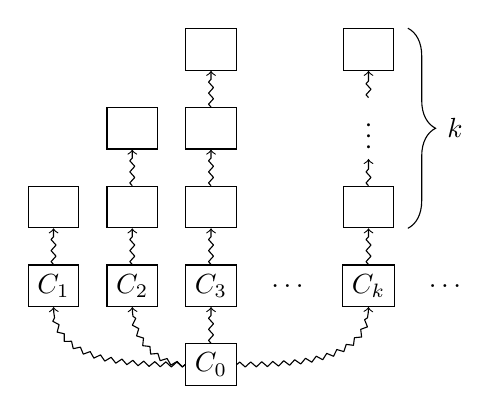
\begin{tikzpicture}[zaggy/.style={line join=round,
decorate, ->,decoration={zigzag, segment length=4,
amplitude=.9,post=lineto, post length=2pt}}]
\node[draw] (c0) at (3,0) {$C_0$};
\node[draw] (c21) at (1,1) {$C_1$};
\node[draw] (c22) at (1,2) {\phantom{$C_0$}};
\node[draw] (c31) at (2,1) {$C_2$};
\node[draw] (c32) at (2,2) {\phantom{$C_0$}};
\node[draw] (c33) at (2,3) {\phantom{$C_0$}};
\node[draw] (c11) at (3,1) {$C_3$};
\node[draw] (c12) at (3,2) {\phantom{$C_0$}};
\node[draw] (c13) at (3,3) {\phantom{$C_0$}};
\node[draw] (c14) at (3,4) {\phantom{$C_0$}};
\node             at (4,1) {$\dots$};
\node[draw] (c41) at (5,1) {$C_k$};
\node[draw] (c42) at (5,2) {\phantom{$C_0$}};
\node       (c43) at (5,3) {$\vdots$};
\node[draw] (c44) at (5,4) {\phantom{$C_0$}};
\node             at (6,1) {$\dots$};
\draw[zaggy] (c0) to [in=270,out=180] (c21);
\draw[zaggy] (c21) -- (c22);
\draw[zaggy] (c0) to [in=270,out=180] (c31);
\draw[zaggy] (c31) -- (c32);
\draw[zaggy] (c32) -- (c33);
\draw[zaggy] (c0) -- (c11);
\draw[zaggy] (c11) -- (c12);
\draw[zaggy] (c12) -- (c13);
\draw[zaggy] (c13) -- (c14);
\draw[zaggy] (c0) to[in=270,out=0] (c41);
\draw[zaggy] (c41) -- (c42);
\draw[zaggy] (c42) -- (c43);
\draw[zaggy] (c43) -- (c44);
\draw[decorate,decoration={brace,amplitude=10pt}]
([xshift=5mm]c44.north) -- ([xshift=5mm]c42.south) node
[black,midway,xshift=6mm] {$k$};
\end{tikzpicture}
\]
Recall that approximant $k$ contains configurations whose traces all
terminate in fewer than $k$ steps. No approximant can contain
configuration $C_0$, since there is no bound on the length of its
traces. Yet this configuration will be admitted by a total correctness
specification whose postcondition is $\mathit{true}$, since it is the
case that each of its traces terminates.

Therefore, in the presence of infinite branching, the fixed point
characterisation of total correctness must be weakened to an
implication. Preservation of greatest lower bounds is unaffected by
infinite branching, so the characterisation of partial correctness
remains intact.

\section{Related work}
\label{sec:related}

Clarke~\cite{clarke79} was the first to study the correspondence
between greatest/least fixed points and partial/total correctness. He
remarks, in a 1979 article, that 
%
\begin{quote}the fixedpoints of $\Gamma$ form a complete
lattice under the natural partial ordering on $\pow(\State)$. The top
element of this lattice is the weakest precondition for partial
correctness and the bottom element is the weakest precondition for
total correctness.~\cite[p.~279, footnote]{clarke79} \end{quote}
%
We note three ways in which the current work extends on Clarke's
original observation. First, Clarke works in the setting of a
particular programming language that provides syntax for sequencing,
conditionals, assignment, and recursive calls to parameterless
procedures. In this paper, we need not tackle issues of programming
language syntax, since we work at the level of arbitrary transition
systems. Second, Clarke's work applies only in a deterministic
setting: a program has either a single final state, or none at all. We
allow for highly non-deterministic programs, and only restrict to
finite non-determinism in the case of total correctness. Third,
Clarke's work is in the setting of a big-step semantics; that is, the
meaning of each programming construct maps an initial state directly
to a final state. We work with a small-step semantics (as described by
a transition system), which means that our approach handles parallel
programs without further adaptation. Big-step semantics is well-known
to be unable to handle parallelism, as acknowledged by Clarke, who
remarks that he `[is] currently attempting to extend this fixedpoint
theory to additional programming features such as
parallelism'~\cite[p.~292]{clarke79}. The definition of total
correctness in a big-step and deterministic setting is trivial, and
hence Clarke's $\Gamma$ functional is straightforward -- this perhaps
explains why Clarke consigned the observation we quote above to a mere
footnote. Our functional, on the other hand, which we call $\SafeOne$,
is fairly subtle: experience shows that even minor modifications of
Definition~\ref{defn:safeone} quickly lead to either the least or the
greatest fixed point becoming degenerate.

Regarding other influences on this work: the idea of using the least
and greatest fixed point of the same function has been previously
exploited by Paulson~\cite[\S3]{paulson97a}, who obtains the set of
finite lists from a function's least fixed point, and the set of
possibly-infinite (`lazy') lists from its greatest fixed point.

Recent work on various Hoare logics for concurrency provide avenues
for further development of the current work. These logics typically
use (mildly disguised) greatest fixed point calculations to obtain a
partial correctness semantics; see, for example,
\cite[Definition~3.2]{vafeiadis11} and
\cite[Definition~25]{dinsdale-young+13}. If these logics were extended
to handle total correctness, the result presented in this paper could
ease the transition.

Another direction for future work is provided by Jacobs and Gries, who
have proposed \emph{general correctness} as a way to unify partial and
total correctness~\cite{jacobs+85}. It would be interesting to
investigate whether general correctness can be also characterised as a
fixed point calculation.
\[
\text{---}
\]
\paragraph{Acknowledgements} This work was supported by EPSRC grant
EP/K011499/1. I would like to thank Edmund Clarke, Alastair Donaldson,
Tony Hoare, Peter Lammich, and Andreas Lochbihler for helpful feedback
and discussions.

\newpage
\bibliographystyle{abbrv}
\bibliography{/Users/jpw48/Dropbox/John}


\end{document}